\section{Results}\label{sec:results}
In this section, the impact assessment for all of the considered test cases from the previous section are developed. With this in mind, two assessments are conducted for each test case. 

Initially, a midpoint assessment is conducted to compare the impact of each note-taking scenario across various environmental mechanisms. This assessment is carried out both comparatively and in absolute terms, aiming to not only highlight the differences in impact between the approaches but also provide context regarding the significance of each category. For instance, while the digital scenario may exhibit a five-times greater impact in a specific category compared to the analog case, if the absolute value remains relatively small, it limits the extent of conclusions that can be drawn from this relationship. In this evaluation, all absolute values are expressed in units such as loss of species per year (species.yr), disability-adjusted life years (DALY), or excess costs in 2013 US Dollars. These units represent the damage to the ecosystem quality, damage to human health, and cost increases due to resource scarcity caused by the note-taking approach, respectively.

Following the midpoint assessment, an endpoint assessment is conducted to establish a single-score comparison between the approaches using normalization factors. This comparison step has a higher level of uncertainty compared to the previous assessment since it requires qualitative input to determine normalization factors across all categories. However, the well-established ReCiPe methodology used in this study provides objectivity to these values to the best of our knowledge.

% Include subsection showing the inventory for both cases maybe

\subsection{Manufacturing Impact}\label{subsec:results_manufacturing}
As mentioned in the previous section, first, the manufacturing processes for both note-taking approaches are compared. For this, the previously mentioned scenarios including their transportation and waste treatments are considered. 

As a first step, their effects per impact category were compared. Figure~\ref{fig:characterization_manufacturing} depicts a relative analysis for the most significant categories between both scenarios while Figure~\ref{fig:characterization_table_manufacturing} shows the absolute values for all impact categories.


\begin{figure}[H]
    \centering
    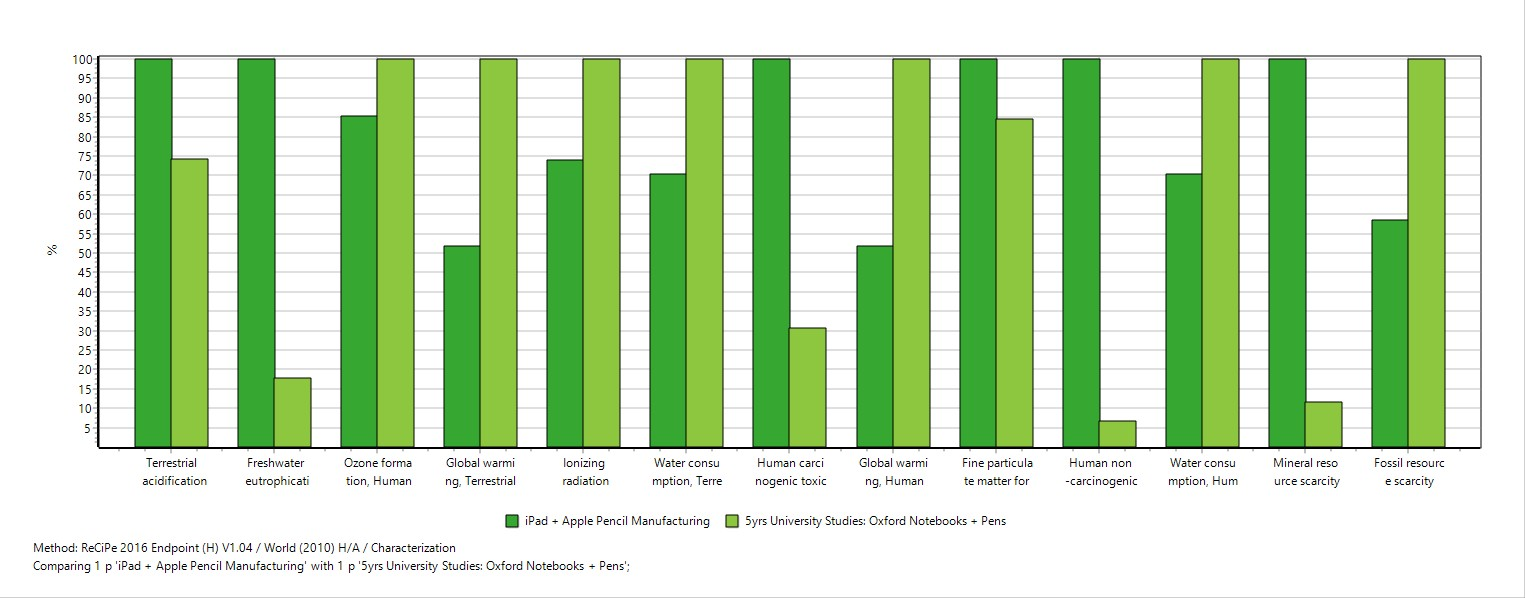
\includegraphics[width=\textwidth]{images/Manufacturing/Characterization_Manufacturing.JPG}
    \caption{Relative midpoint assessment for the manufacturing of the investigated note-taking approaches per impact category.}\label{fig:characterization_manufacturing}
\end{figure}

This Figure showcases the similarity between the impact for both note-taking scenarios where each case dominates six categories. However, a clear disparity favoring the digital approach can be seen for all categories related with global warming and natural resources. The analog case causes about twice as much global warming on average over the three considered categories and is well above the digital case for scarcity of fossil resources, water consumption and ozone formation. On the other hand, the digital case has a much greater impact in categories involving the damaging of ecosystems such as terrestrial acidification and freshwater eutrophication as well as human impacts (carcinogenic and non-carcinogenic) and scarcity of mineral resources.

\begin{figure}[H]
    \centering
    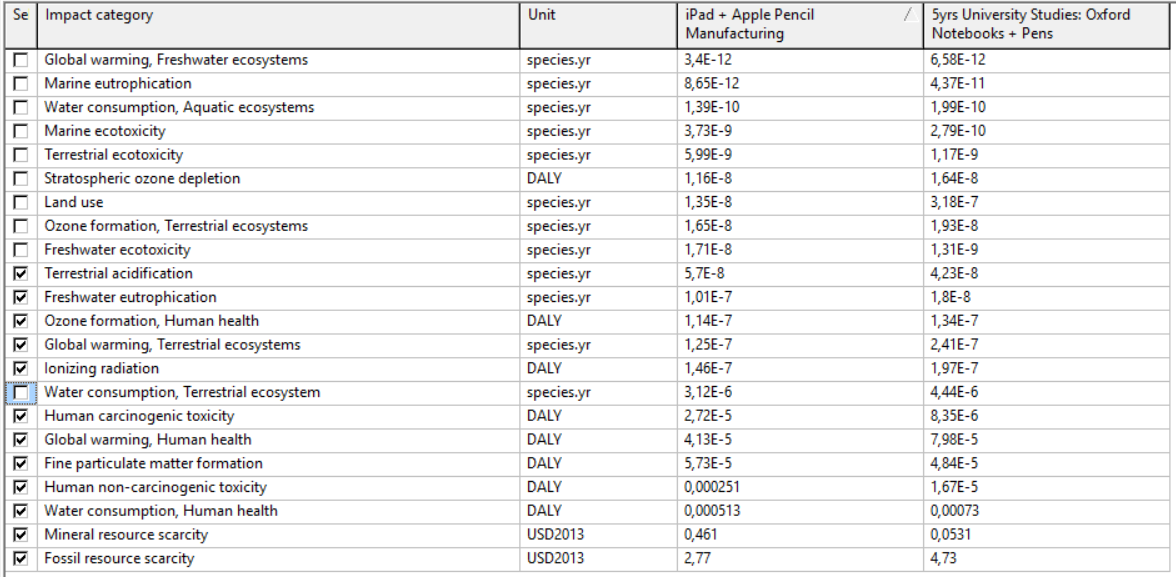
\includegraphics[width=0.9\textwidth]{images/Manufacturing/Characterization_Table_Manufacturing.PNG}
    \caption{Absolute midpoint assessment for the manufacturing of the investigated note-taking approaches per impact category.}\label{fig:characterization_table_manufacturing}
\end{figure}

From Figure~\ref{fig:characterization_table_manufacturing}, the same trend is observed. Terrestrial ecotoxicity caused by the digital case is more than five times larger than for the analog case, whereas the land use for the analog case is an entire order of magnitude larger than the digital case. Nevertheless, these remaining categories are orders of magnitude smaller than the ones described in the previous Figure and must be carefully analyzed as to not allow for the attention to be deviated from the impact categories with the majority of the impact share. 

Once the midpoint assessment is conducted, the impact categories can be divided into three main groups based on the recipient for their impacts: the ecosystem, human health and the global resources. Figure~\ref{fig:damage_assessment_manufacturing} showcases a relative comparison per category between both note-taking scenarios.

\begin{figure}[H]
    \centering
    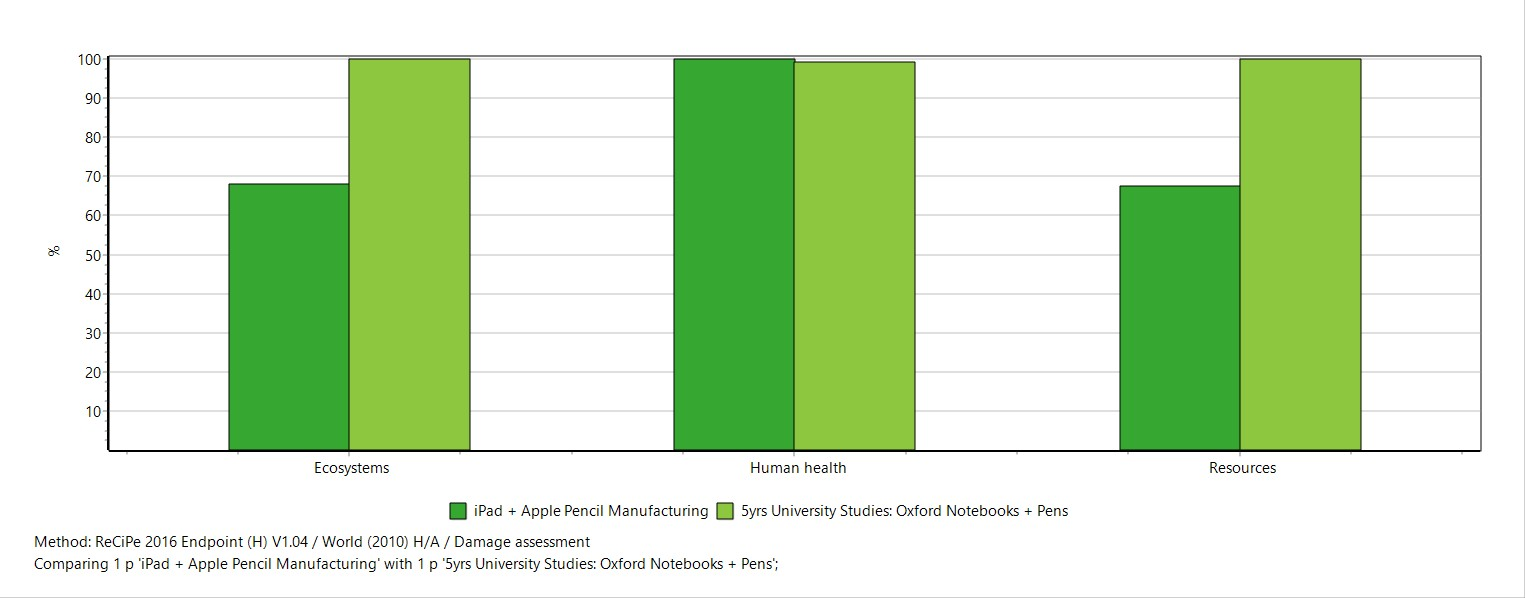
\includegraphics[width=\textwidth]{images/Manufacturing/Damage_Assessment_Manufacturing.JPG}
    \caption{Relative endpoint assessment for the manufacturing of the investigated note-taking approaches.}\label{fig:damage_assessment_manufacturing}
\end{figure}

Based on these findings, it is apparent that both manufacturing processes exhibit a comparable impact on human health, with a slight advantage observed for the digital scenario. However, the analog scenario demonstrates approximately a 40\% greater impact on the ecosystem and global resources. This discovery is particularly unexpected, considering the significant manufacturing requirements and intercontinental transportation involved in the digital scenario.

Nevertheless, similar to the midpoint assessment, analyzing the absolute scores for each category is imperative for the context of this difference. Figure~\ref{fig:single_score_manufacturing} depicts the total single score given to the manufacturing for both note-taking scenarios alongside their internal distributions. 

\begin{figure}[H]
    \centering
    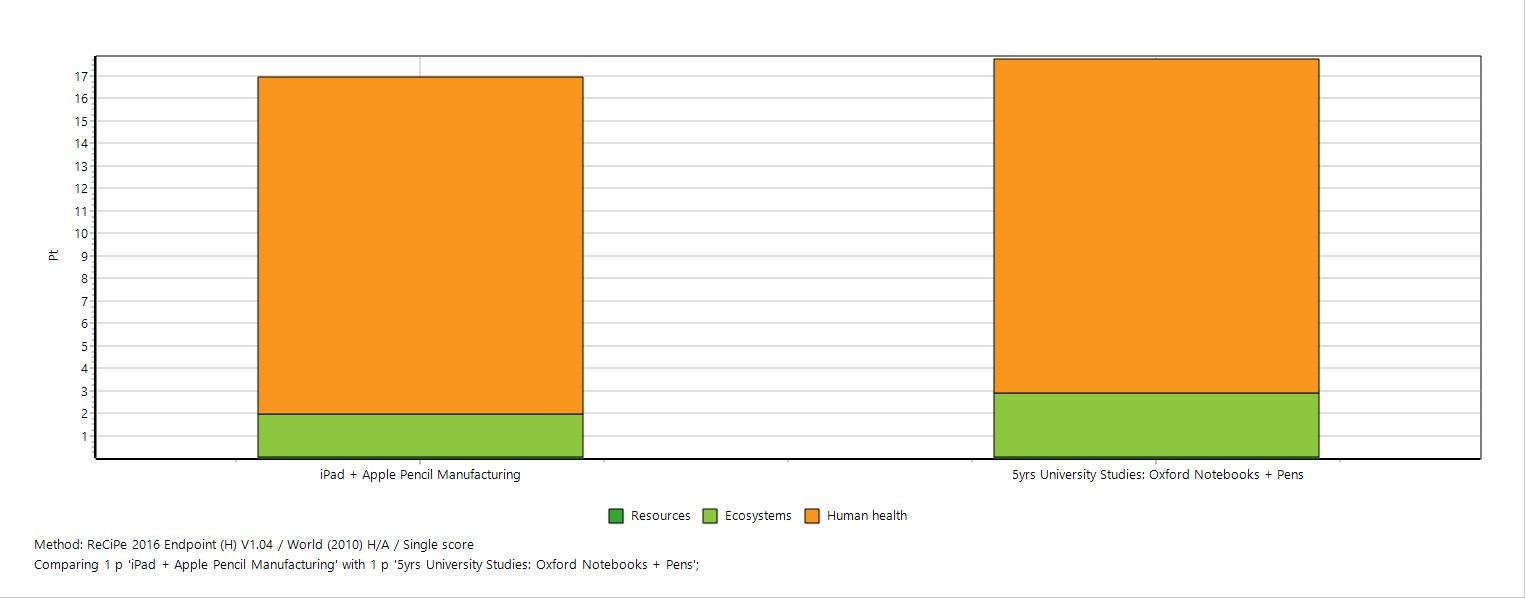
\includegraphics[width=\textwidth]{images/Manufacturing/Single_Score_Manufacturing.JPG}
    \caption{Single score distribution for the manufacturing of the investigated note-taking approaches.}\label{fig:single_score_manufacturing}
\end{figure}

From here, it becomes evident that the impact on human health is the major contributor for both scenarios, with the 40\% increase in ecosystem and resource impact for the analog scenario amounting to a surplus of an individual single score point. 

\subsection{Life Cycle Impact}\label{subsec:results_life_cycle}
Once the manufacturing for both note-taking scenarios was compared, the energy required to power the electronics from the digital case are taken into account. As mentioned earlier, three energy source scenarios are considered ranging from 0 to 100\% RES penetration for the grid mix. The results for their midpoint and endpoint assessment comparisons are seen in the following.

\subsubsection{0\% RES Penetration}\label{subsubsec:0RES}
As expected, the impact for the digital case increases massively when the energy required to charge and operate the electronics is considered. Figures~\ref{fig:characterization_RES_0} and~\ref{fig:characterization_table_RES_0} showcase the midpoint assessment for both scenarios with 0\% RES penetration.

\begin{figure}[H]
    \centering
    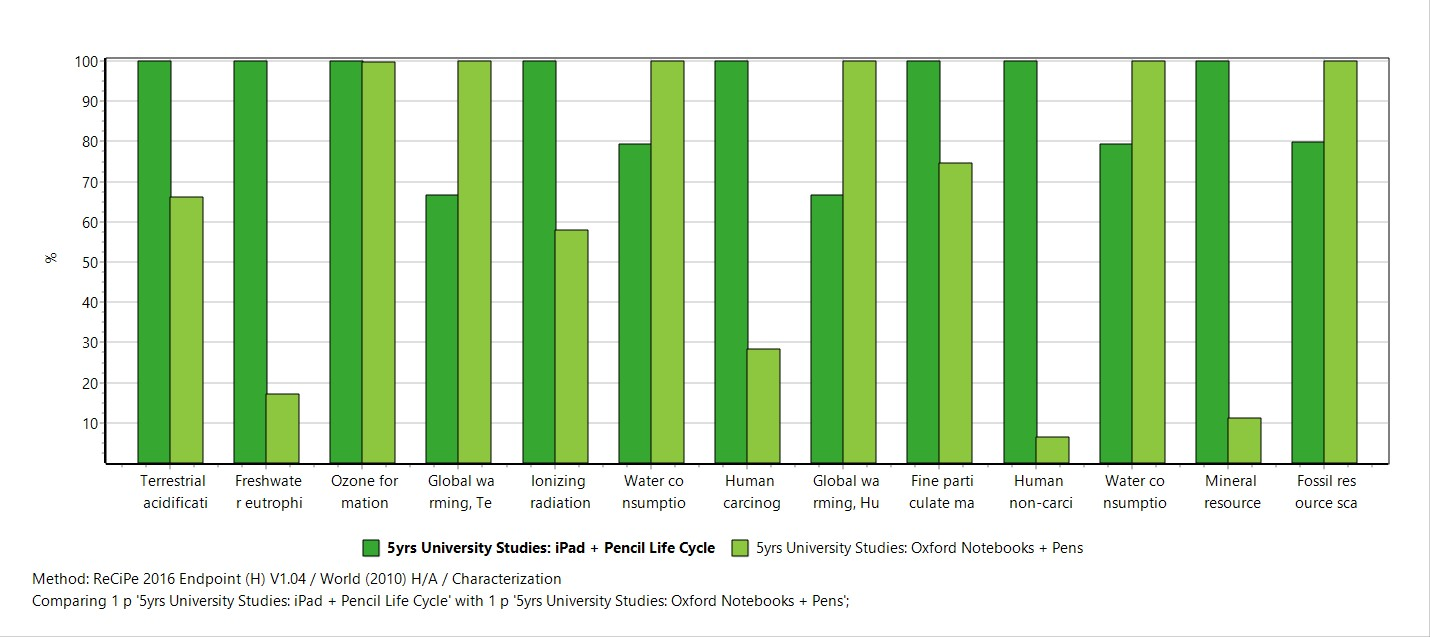
\includegraphics[width=\textwidth]{images/RES_0/Characterization_RES_0.JPG}
    \caption{Relative midpoint assessment for a 0\% RES penetration scenario.}\label{fig:characterization_RES_0}
\end{figure}

From Figure~\ref{fig:characterization_RES_0} it becomes evident that the impact caused by the energy required to run the electronics causes for the digital case to far outweigh the impact for the analog case. The analog case represents no more than 20\% of the impact caused by the digital case across all categories, with most being below 15\%.

\begin{figure}[H]
    \centering
    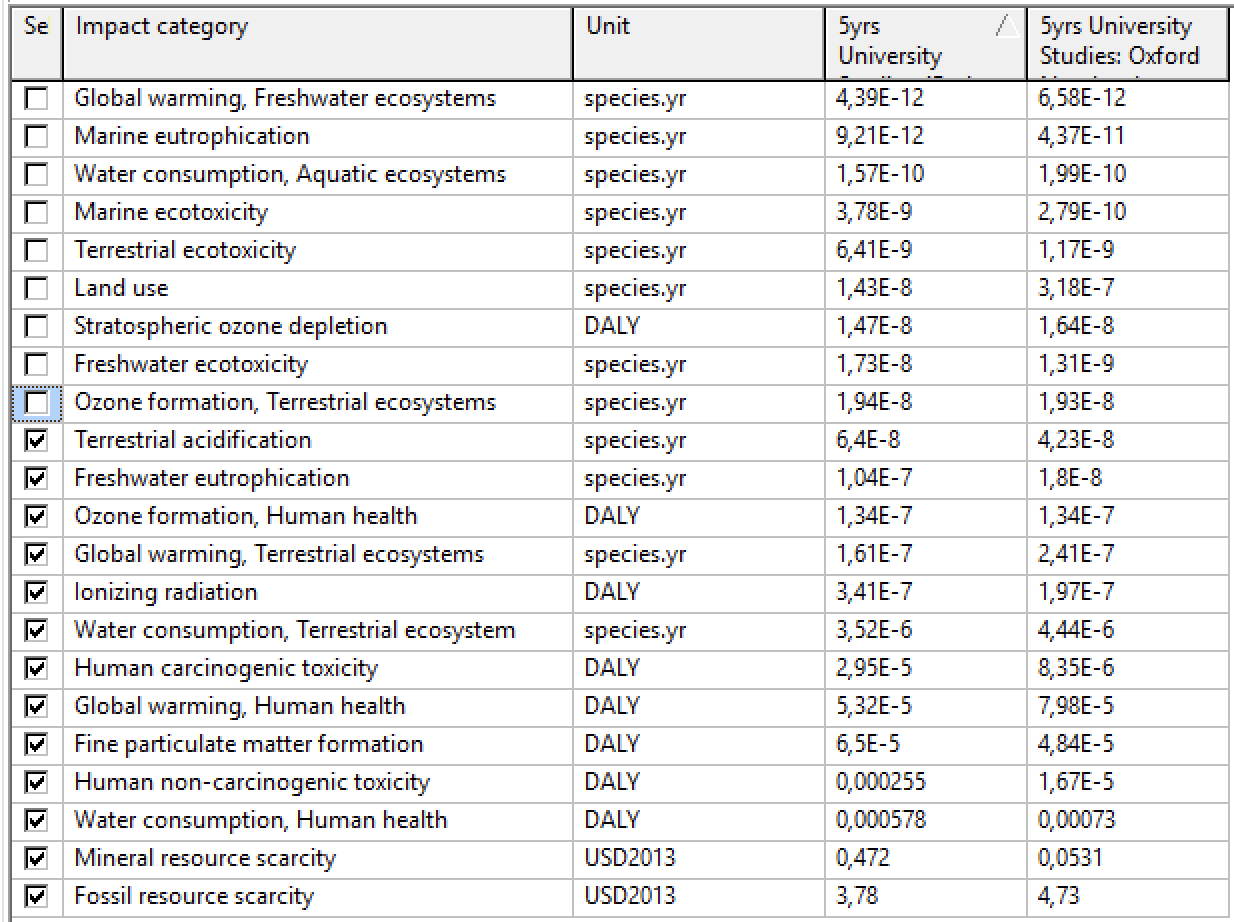
\includegraphics[width=0.9\textwidth]{images/RES_0/Characterization_Table_RES_0.PNG}
    \caption{Absolute midpoint assessment for a 0\% RES penetration scenario.}\label{fig:characterization_table_RES_0}
\end{figure}

Analyzing the endpoint assessment for both scenarios in Figures~\ref{fig:damage_assessment_RES_0} and~\ref{fig:single_score_RES0} showcases the same behavior. It becomes clear that the driving force for the impact of the digital scenario is the energy required to charge the electronics.

\begin{figure}[H]
    \centering
    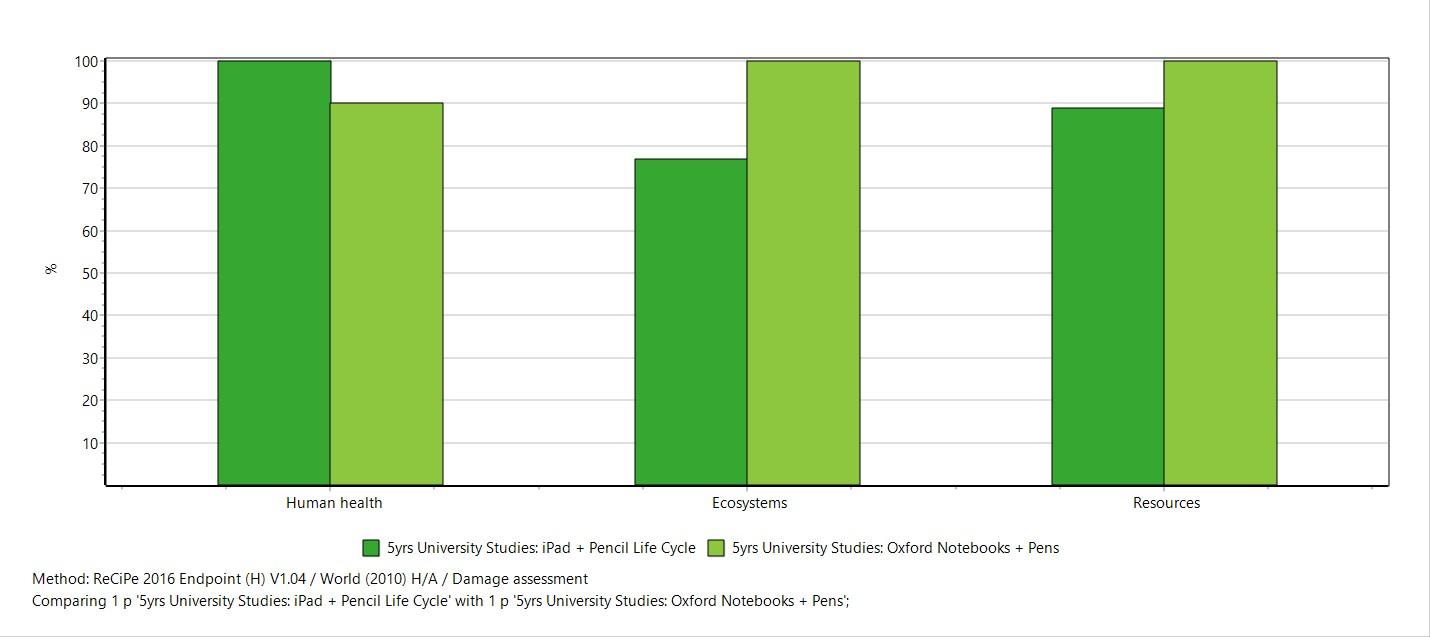
\includegraphics[width=\textwidth]{images/RES_0/Damage_Assessment_RES_0.JPG}
    \caption{Relative endpoint assessment for a 0\% RES penetration scenario.}\label{fig:damage_assessment_RES_0}
\end{figure}

By comparing the single score for the digital case before and after considering the electricity required to power it, a steep rise for its single score of 68 ecopoints is observed. This represents a 500\% increase for its single score, mainly driven by its human health factor, accounting for approximately 87\% of the score and secondly by its impact on the ecosystem, accounting for approximately 13\% of the score. 

\begin{figure}[H]
    \centering
    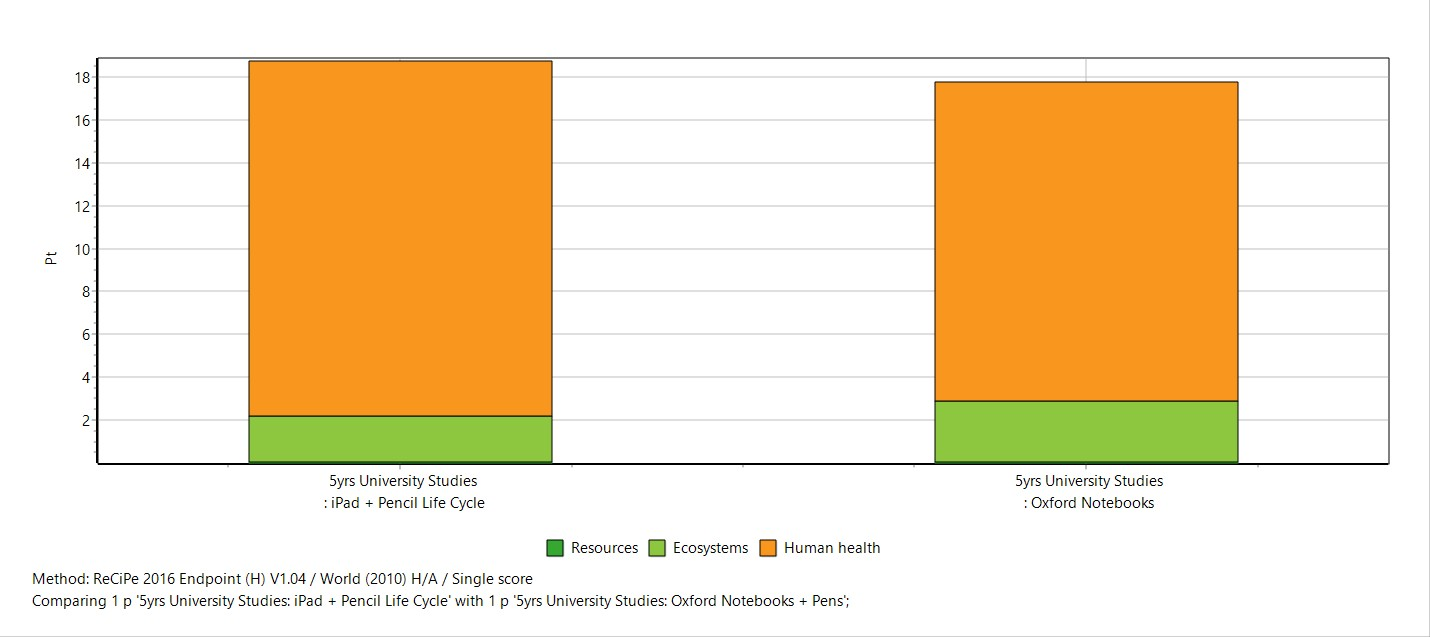
\includegraphics[width=\textwidth]{images/RES_0/Single_Score_RES_0.JPG}
    \caption{Single score distribution for a 0\% RES penetration scenario.}\label{fig:single_score_RES0}
\end{figure}

\subsubsection{50\% RES Penetration}

The second energy source scenario depicts a 50\% RES penetration. Figure \ref*{fig:characterization_RES_50} shows the relative midpoint assessment for the two note-taking alternatives considered, while Figure \ref{fig:characterization_table_RES_50} depicts the categories considered alongside their absolute midpoint assessment values. The results are similar to those presented in Subsection \ref{subsubsec:0RES}, where clearly the analog alternative has a lower impact per category. Nevertheless, some categories have increased for the 50\% RES in comparison to the 0\% RES. For instance, the \textit{ozone formation for human health} category had a relative increase of around 6\% for the analog case. Similarly, both \textit{global warming} categories considered present a relative increase of 10\%. These can be attributed to the reduction in impact for the digital case compared to the 0\% RES scenario over these categories. On the other hand, \textit{water consumption} for human health and terrestrial ecosystems presented a relative impact reduction of 7\% and 9\%, respectively, attributed to an increase for the impact in the digital case with respect to the 0\% RES scenario. 

\begin{figure}[H]
    \centering
    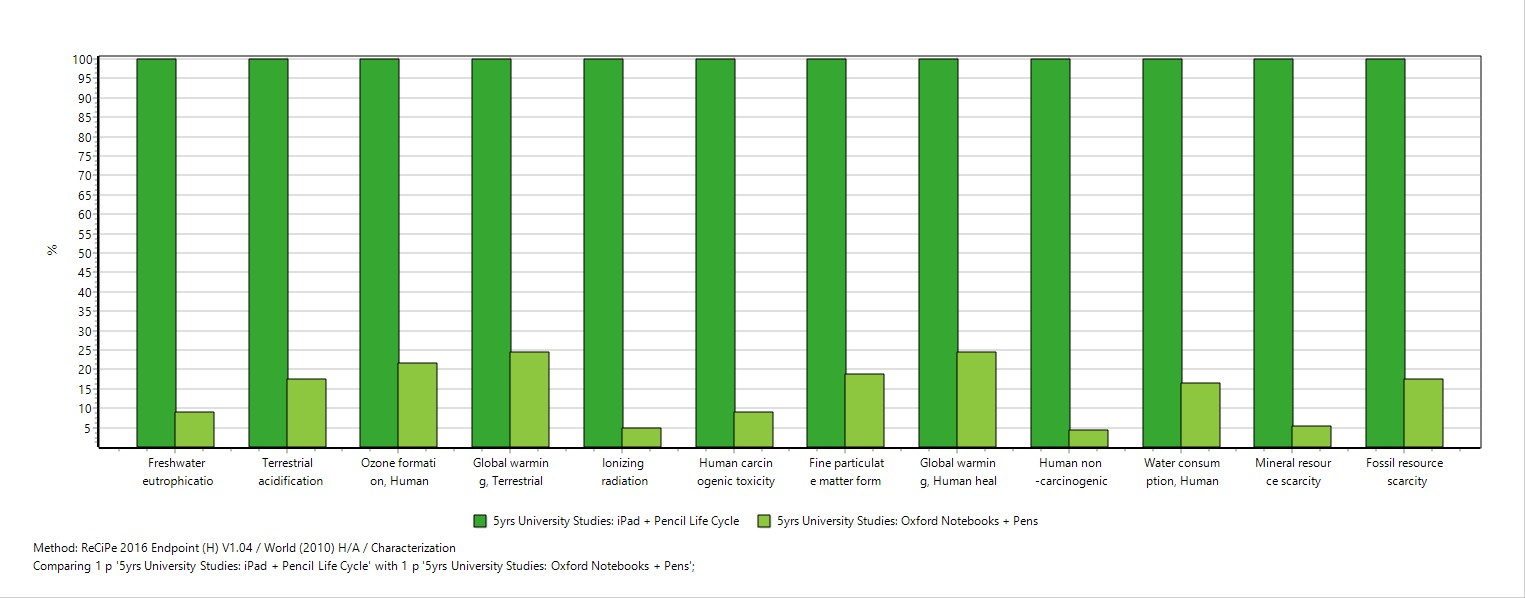
\includegraphics[width=\textwidth]{images/RES_50/Characterization_RES_50.JPG}
    \caption{Relative midpoint assessment for a 50\% RES penetration scenario.}\label{fig:characterization_RES_50}
\end{figure}

\begin{figure}[H]
    \centering
    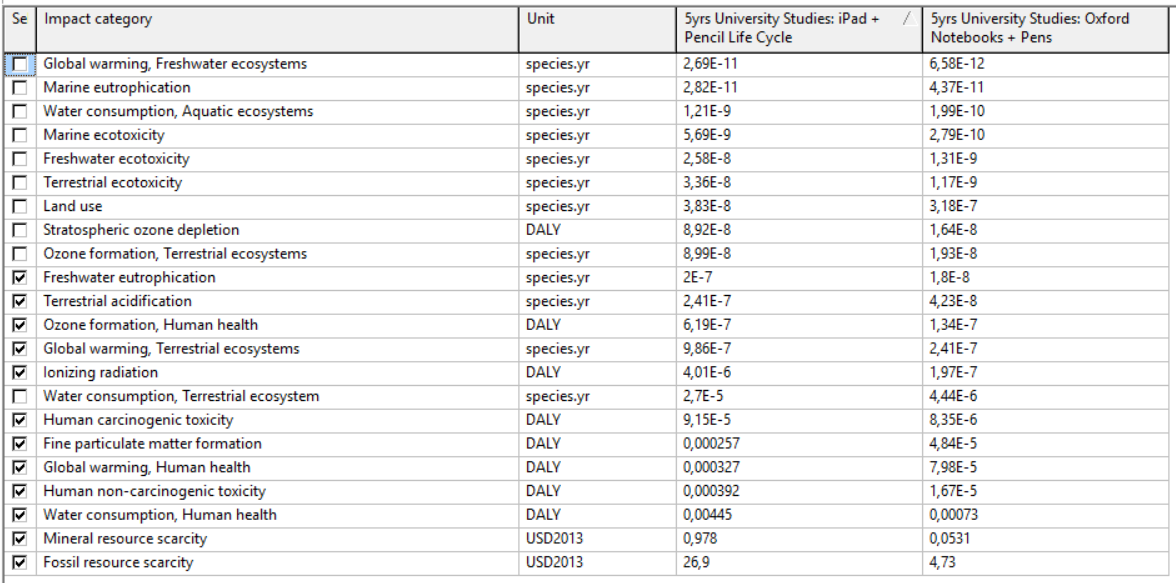
\includegraphics[width=0.9\textwidth]{images/RES_50/Characterization_Table_RES_50.PNG}
    \caption{Absolute midpoint assessment for a 50\% RES penetration scenario.}\label{fig:characterization_table_RES_50}
\end{figure}

The relative endpoint assessment per impact category of the 50\% RES scenario for the note-taking methods is shown in Figure \ref{fig:damage_assessment_RES_50}. In contrast with the 0\% RES scenario, the \textit{ecosystems} and \textit{human health} impacts are lower for this case, with 6\% and 2\% reductions, respectively. However, the \textit{resources} category increased by 8\% for the 50\% RES scenario. These results indicate that, between the 0\% RES scenario and the 50\% RES scenario, an increase for the ecosystem and human health impacts from part of the digital case are experienced, alongside a decrease in the impact over resources.  

\begin{figure}[H]
    \centering
    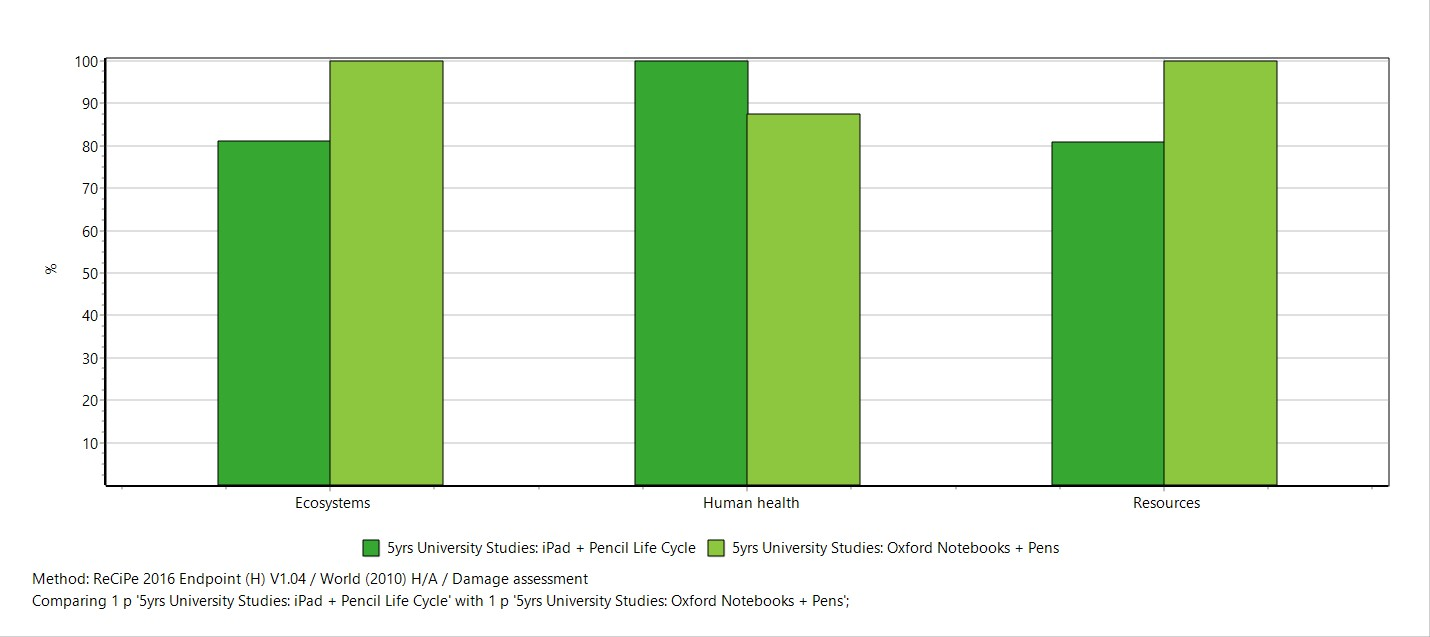
\includegraphics[width=\textwidth]{images/RES_50/Damage_Assessment_RES_50.JPG}
    \caption{Relative endpoint assessment for a 50\% RES scenario.}\label{fig:damage_assessment_RES_50}
\end{figure}

By analyzing the total single score given for the 50\% RES scenario for both note-taking options in Figure \ref{fig:single_score_RES50}, it can be observed that the \textit{human health} category has the biggest impact over the \textit{ecosystem} and \textit{resources} categories for the analog and digital note-taking approaches. Moreover, an increase for the single score given to the digital case of approximately 25 ecopoints is observed. This was not expected since, in general, a higher RES results in lower impacts. However, for this application, it seems that the increase in water consumption between both scenarios (0.00302 DALY for 0\% RES and 0.00445 DALY for 50\% RES) is the driving factor for this increase as in every other human health factor, the 0\% RES scenario shows larger values. Nevertheless, the impact of this increased water consumption results in an increase of about 18 ecopoints for its single score rating in the human health category.

\begin{figure}[H]
    \centering
    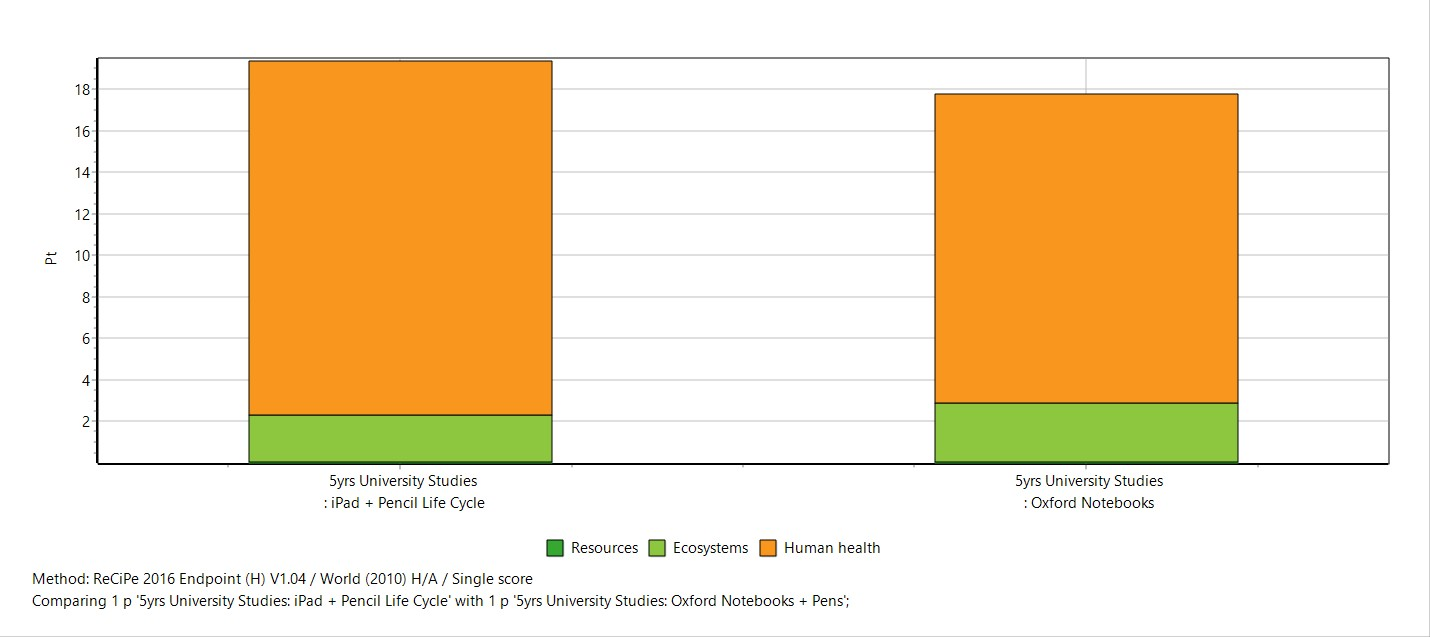
\includegraphics[width=\textwidth]{images/RES_50/Single_Score_RES_50.JPG}
    \caption{Single score distribution for a 50\% RES penetration scenario.}\label{fig:single_score_RES50}
\end{figure}

Comparing these findings to the relatively even results from the manufacturing comparison, it can be concluded that the main driving factor for the digital case's impact is its energy source. For this reason, scenarios with increasing RES shares are investigated in the following.

\subsubsection{100\% RES Penetration}

The last energy scenario consists of defining a 100\% RES penetration to charge the digital note-taking method, which means that all the energy comes from renewable sources. Figure \ref{fig:characterization_RES_100} shows the relative midpoint assessment for both note-taking methods, and Figure \ref{fig:characterization_table_RES_100} the relevant impact categories alongside their absolute midpoint assessment. Since now the energy sources are completely renewable, it would be logical to expect a lower impact in some categories from the digital alternative. In contrast to the 50\% RES, the \textit{ozone formation} for human health, and \textit{global warming} categories present a relative increase for the analog alternative, meaning that a decrease for the digital scenario was experienced. The \textit{ozone formation} increased 16\%, while the \textit{global warming} for terrestrial ecosystems and human health presented the largest change, with a 26\% and 28\% increase respectively. This means that the digital note-taking alternative contributes less to global warming than the analog option, according to its midpoint assessment. On the other hand the \textit{water consumption} impact stayed relatively the same for the 100\% RES penetration scenario.

\begin{figure}[H]
    \centering
    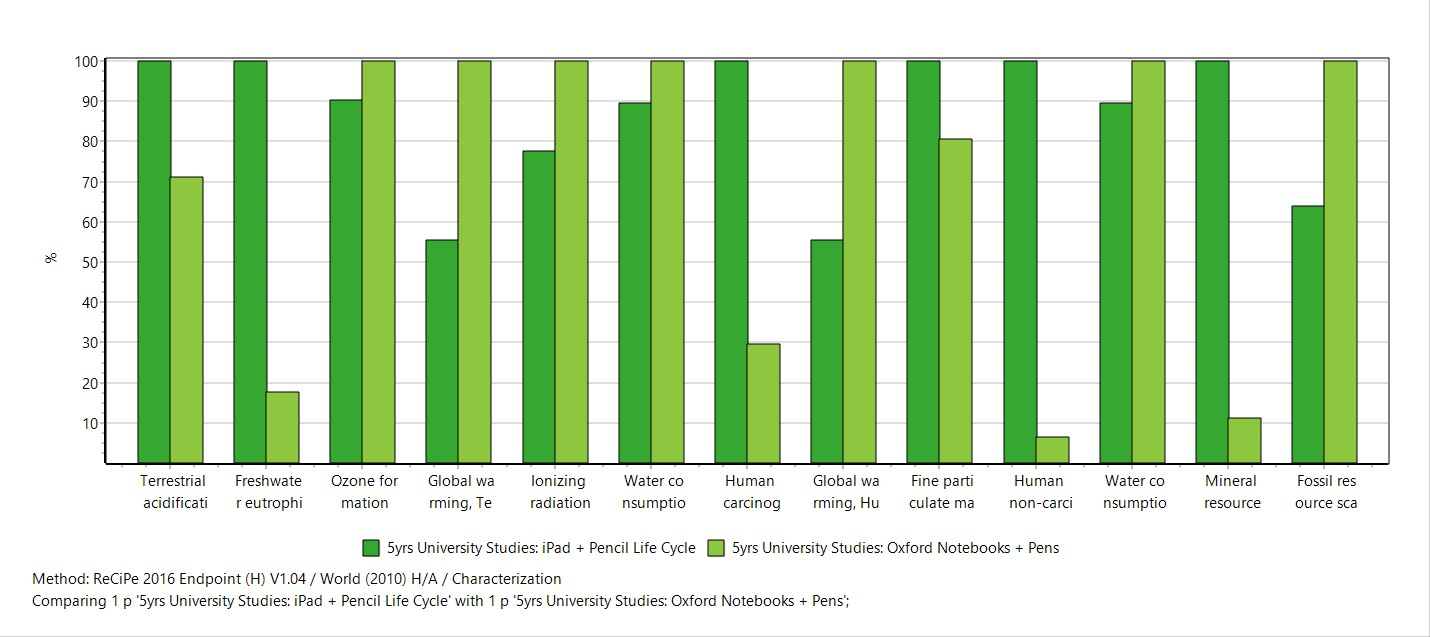
\includegraphics[width=\textwidth]{images/RES_100/Characterization_RES_100.JPG}
    \caption{Relative midpoint assessment for a 100\% RES penetration scenario.}\label{fig:characterization_RES_100}
\end{figure}

\begin{figure}[H]
    \centering
    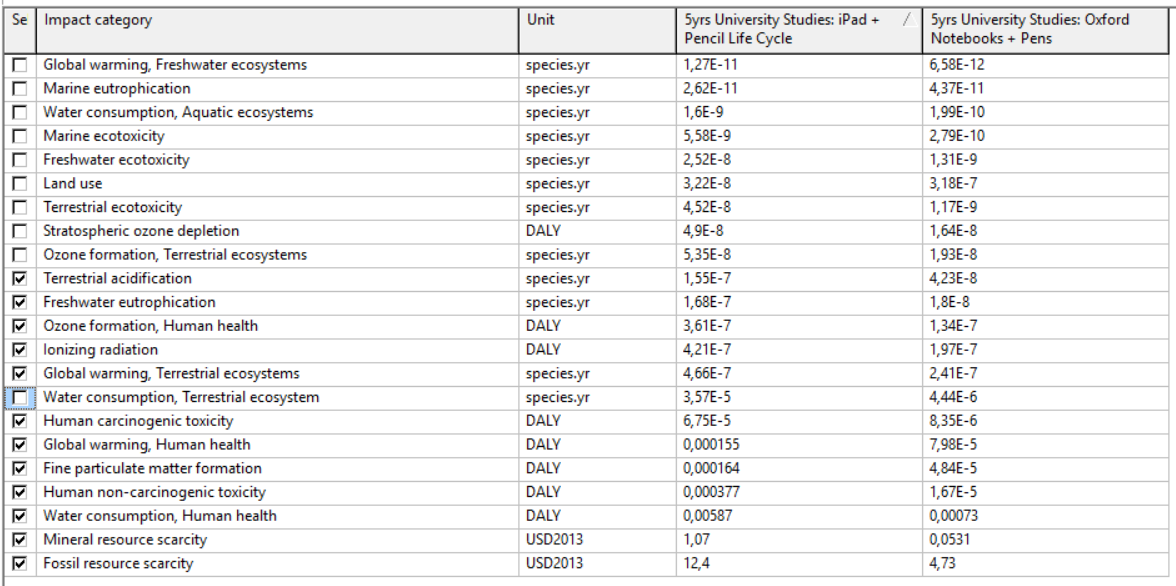
\includegraphics[width=0.9\textwidth]{images/RES_100/Characterization_Table_RES_100.PNG}
    \caption{Absolute midpoint assessment for a 100\% RES penetration scenario.}\label{fig:characterization_table_RES_100}
\end{figure}

Figure \ref{fig:damage_assessment_RES_100} shows the endpoint assessment of 100\% RES scenario for the note-taking methods considered. The impact in \textit{human health} and \textit{resources} dropped 4\% in for the analog alternative if compared to the 50\% RES scenario. On the other hand, the ecosystem impact increased 19\% for the analog case, which means that the impact of the digital note-taking method is definitely lower with completely renewable energy sources. Nevertheless, the ecosystem of the digital alternative is still considerably higher than the analog option. 

\begin{figure}[H]
    \centering
    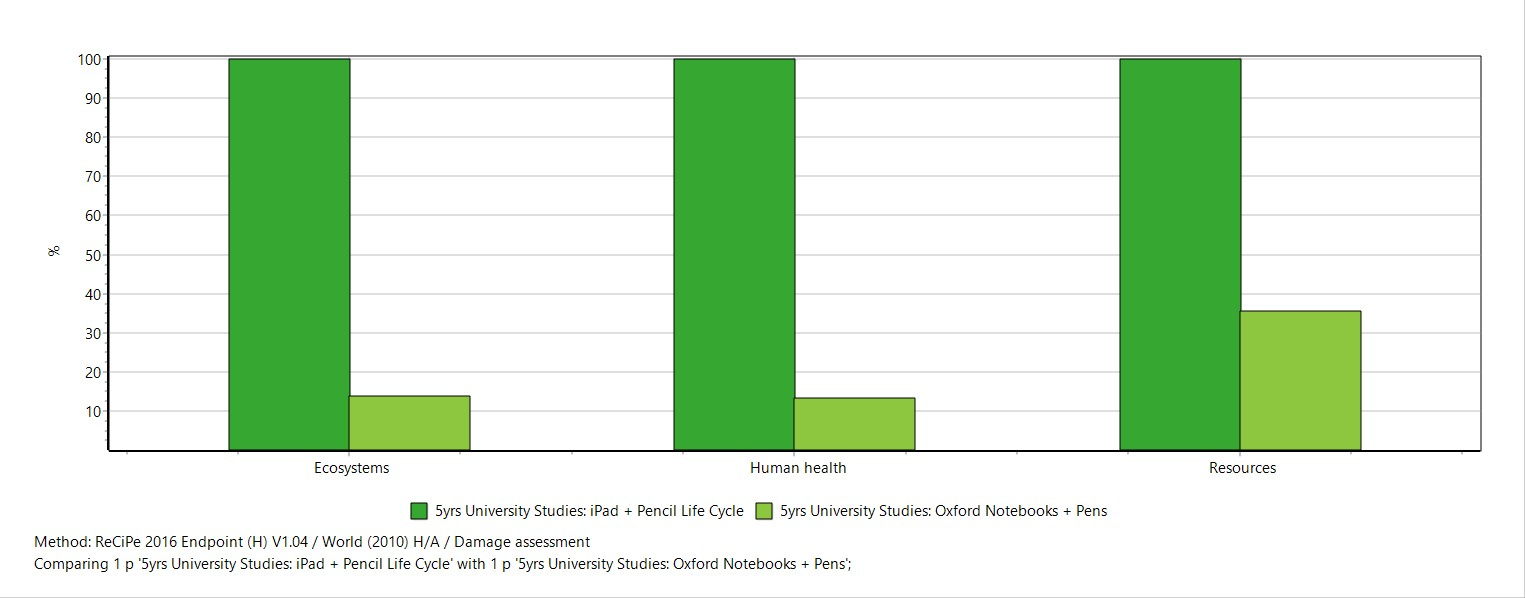
\includegraphics[width=\textwidth]{images/RES_100/Damage_Assessment_RES_100.JPG}
    \caption{Relative endpoint assessment for a 50\% RES scenario.}\label{fig:damage_assessment_RES_100}
\end{figure}

Figure \ref{fig:single_score_RES100} shows the total single score given for the 100\% RES energy scenario. Comparing these results to the ones seen for the 50\% RES scenario, an absolute increase can be seen for the single score for the digital scenario. Again, this is attributed to the effects of water consumption on human health, given that all other categories are actually lower, similar to the last case. This increase in water consumption accounts for approximately a 19 point increase between both scenarios. 

\begin{figure}[H]
    \centering
    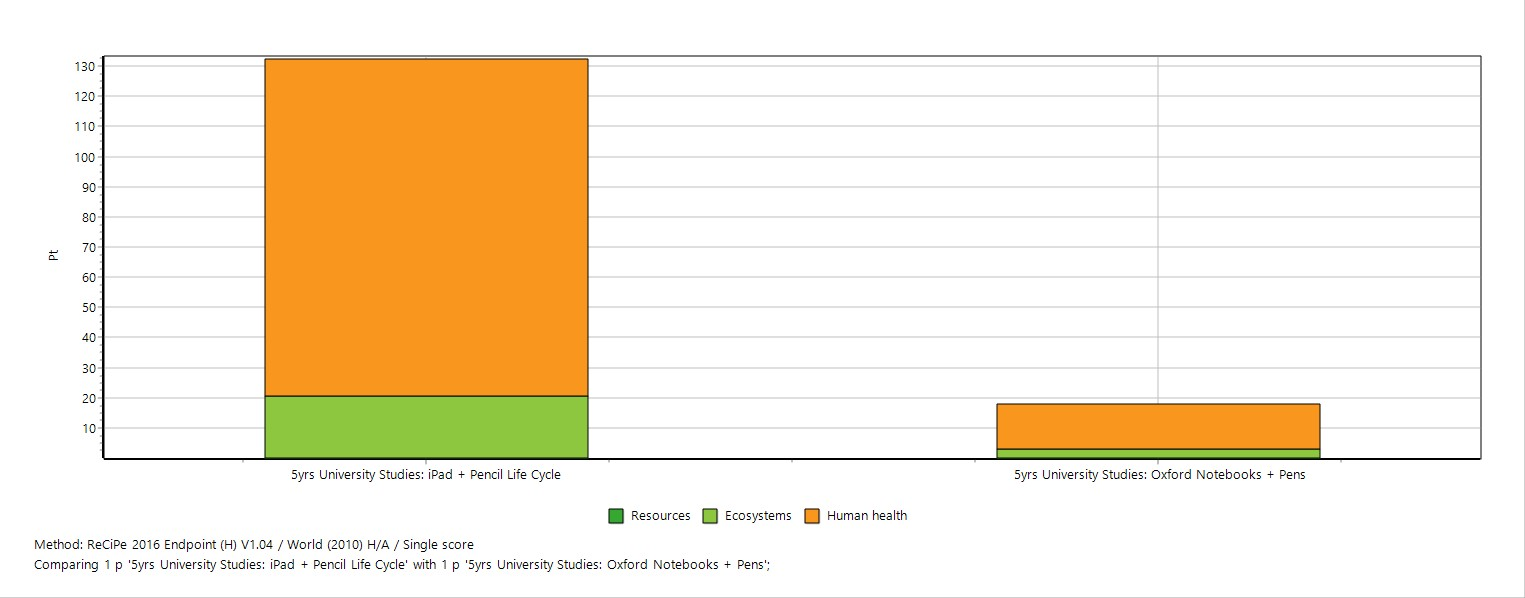
\includegraphics[width=\textwidth]{images/RES_100/Single_Score_RES_100.JPG}
    \caption{Single score distribution for a 100\% RES scenario.}\label{fig:single_score_RES100}
\end{figure}